\documentclass[11pt,ignorenonframetext,]{beamer}
\setbeamertemplate{caption}[numbered]
\setbeamertemplate{caption label separator}{: }
\setbeamercolor{caption name}{fg=normal text.fg}
\beamertemplatenavigationsymbolsempty
\usepackage{lmodern}
\usepackage{amssymb,amsmath}
\usepackage{ifxetex,ifluatex}
\usepackage{fixltx2e} % provides \textsubscript
\ifnum 0\ifxetex 1\fi\ifluatex 1\fi=0 % if pdftex
  \usepackage[T1]{fontenc}
  \usepackage[utf8]{inputenc}
\else % if luatex or xelatex
  \ifxetex
    \usepackage{mathspec}
  \else
    \usepackage{fontspec}
  \fi
  \defaultfontfeatures{Ligatures=TeX,Scale=MatchLowercase}
\fi
\usetheme[]{metropolis}
% use upquote if available, for straight quotes in verbatim environments
\IfFileExists{upquote.sty}{\usepackage{upquote}}{}
% use microtype if available
\IfFileExists{microtype.sty}{%
\usepackage{microtype}
\UseMicrotypeSet[protrusion]{basicmath} % disable protrusion for tt fonts
}{}
\newif\ifbibliography
\hypersetup{
            pdftitle={Lecture 3},
            pdfauthor={Colin Rundel},
            pdfborder={0 0 0},
            breaklinks=true}
\usepackage{color}
\usepackage{fancyvrb}
\newcommand{\VerbBar}{|}
\newcommand{\VERB}{\Verb[commandchars=\\\{\}]}
\DefineVerbatimEnvironment{Highlighting}{Verbatim}{commandchars=\\\{\}}
% Add ',fontsize=\small' for more characters per line
\newenvironment{Shaded}{}{}
\newcommand{\KeywordTok}[1]{\textcolor[rgb]{0.00,0.44,0.13}{\textbf{{#1}}}}
\newcommand{\DataTypeTok}[1]{\textcolor[rgb]{0.56,0.13,0.00}{{#1}}}
\newcommand{\DecValTok}[1]{\textcolor[rgb]{0.25,0.63,0.44}{{#1}}}
\newcommand{\BaseNTok}[1]{\textcolor[rgb]{0.25,0.63,0.44}{{#1}}}
\newcommand{\FloatTok}[1]{\textcolor[rgb]{0.25,0.63,0.44}{{#1}}}
\newcommand{\ConstantTok}[1]{\textcolor[rgb]{0.53,0.00,0.00}{{#1}}}
\newcommand{\CharTok}[1]{\textcolor[rgb]{0.25,0.44,0.63}{{#1}}}
\newcommand{\SpecialCharTok}[1]{\textcolor[rgb]{0.25,0.44,0.63}{{#1}}}
\newcommand{\StringTok}[1]{\textcolor[rgb]{0.25,0.44,0.63}{{#1}}}
\newcommand{\VerbatimStringTok}[1]{\textcolor[rgb]{0.25,0.44,0.63}{{#1}}}
\newcommand{\SpecialStringTok}[1]{\textcolor[rgb]{0.73,0.40,0.53}{{#1}}}
\newcommand{\ImportTok}[1]{{#1}}
\newcommand{\CommentTok}[1]{\textcolor[rgb]{0.38,0.63,0.69}{\textit{{#1}}}}
\newcommand{\DocumentationTok}[1]{\textcolor[rgb]{0.73,0.13,0.13}{\textit{{#1}}}}
\newcommand{\AnnotationTok}[1]{\textcolor[rgb]{0.38,0.63,0.69}{\textbf{\textit{{#1}}}}}
\newcommand{\CommentVarTok}[1]{\textcolor[rgb]{0.38,0.63,0.69}{\textbf{\textit{{#1}}}}}
\newcommand{\OtherTok}[1]{\textcolor[rgb]{0.00,0.44,0.13}{{#1}}}
\newcommand{\FunctionTok}[1]{\textcolor[rgb]{0.02,0.16,0.49}{{#1}}}
\newcommand{\VariableTok}[1]{\textcolor[rgb]{0.10,0.09,0.49}{{#1}}}
\newcommand{\ControlFlowTok}[1]{\textcolor[rgb]{0.00,0.44,0.13}{\textbf{{#1}}}}
\newcommand{\OperatorTok}[1]{\textcolor[rgb]{0.40,0.40,0.40}{{#1}}}
\newcommand{\BuiltInTok}[1]{{#1}}
\newcommand{\ExtensionTok}[1]{{#1}}
\newcommand{\PreprocessorTok}[1]{\textcolor[rgb]{0.74,0.48,0.00}{{#1}}}
\newcommand{\AttributeTok}[1]{\textcolor[rgb]{0.49,0.56,0.16}{{#1}}}
\newcommand{\RegionMarkerTok}[1]{{#1}}
\newcommand{\InformationTok}[1]{\textcolor[rgb]{0.38,0.63,0.69}{\textbf{\textit{{#1}}}}}
\newcommand{\WarningTok}[1]{\textcolor[rgb]{0.38,0.63,0.69}{\textbf{\textit{{#1}}}}}
\newcommand{\AlertTok}[1]{\textcolor[rgb]{1.00,0.00,0.00}{\textbf{{#1}}}}
\newcommand{\ErrorTok}[1]{\textcolor[rgb]{1.00,0.00,0.00}{\textbf{{#1}}}}
\newcommand{\NormalTok}[1]{{#1}}
\usepackage{graphicx,grffile}
\makeatletter
\def\maxwidth{\ifdim\Gin@nat@width>\linewidth\linewidth\else\Gin@nat@width\fi}
\def\maxheight{\ifdim\Gin@nat@height>\textheight0.8\textheight\else\Gin@nat@height\fi}
\makeatother
% Scale images if necessary, so that they will not overflow the page
% margins by default, and it is still possible to overwrite the defaults
% using explicit options in \includegraphics[width, height, ...]{}
\setkeys{Gin}{width=\maxwidth,height=\maxheight,keepaspectratio}

% Prevent slide breaks in the middle of a paragraph:
\widowpenalties 1 10000
\raggedbottom

\AtBeginPart{
  \let\insertpartnumber\relax
  \let\partname\relax
  \frame{\partpage}
}
\AtBeginSection{
  \ifbibliography
  \else
    \let\insertsectionnumber\relax
    \let\sectionname\relax
    \frame{\sectionpage}
  \fi
}
\AtBeginSubsection{
  \let\insertsubsectionnumber\relax
  \let\subsectionname\relax
  \frame{\subsectionpage}
}

\setlength{\parindent}{0pt}
\setlength{\parskip}{6pt plus 2pt minus 1pt}
\setlength{\emergencystretch}{3em}  % prevent overfull lines
\providecommand{\tightlist}{%
  \setlength{\itemsep}{0pt}\setlength{\parskip}{0pt}}
\setcounter{secnumdepth}{0}

\usepackage{geometry}
\usepackage{graphicx}
\usepackage{amssymb}
\usepackage{color}          	% gives color options
\usepackage{url}		% produces hyperlinks
\usepackage[english]{babel}
\usepackage{colortbl}	% allows for color usage in tables
\usepackage{multirow}	% allows for rows that span multiple rows in tables
\usepackage{xcolor}		% this package has a variety of color options
\usepackage{calc}
\usepackage{multicol}
\usepackage{wrapfig}
\usepackage{textcomp}
\usepackage{bm}
\usepackage{bbm}
\usepackage{setspace}
\singlespacing

%%%%%%%%%%%%%%%%
% Small code output
%%%%%%%%%%%%%%%%

%% change fontsize of R code
\let\oldShaded\Shaded
\let\endoldShaded\endShaded
\renewenvironment{Shaded}{\footnotesize\begin{spacing}{0.9}\oldShaded}{\endoldShaded\end{spacing}}

%% change fontsize of output
\let\oldverbatim\verbatim
\let\endoldverbatim\endverbatim
\renewenvironment{verbatim}{\footnotesize\begin{spacing}{0.9}\oldverbatim}{\endoldverbatim\end{spacing}}


%%%%%%%%%%%%%%%%
% Custom Colors
%%%%%%%%%%%%%%%%

\xdefinecolor{oiBlue}{rgb}{0.15, 0.35, 0.55}
\xdefinecolor{gray}{rgb}{0.5, 0.5, 0.5}
\xdefinecolor{darkGray}{rgb}{0.3, 0.3, 0.3}
\xdefinecolor{darkerGray}{rgb}{0.2, 0.2, 0.2}
\xdefinecolor{rubineRed}{rgb}{0.89,0,0.30}
\xdefinecolor{linkCol}{rgb}{0.11,0.49,0.95}	
\xdefinecolor{irishGreen}{rgb}{0,0.60,0}	
\xdefinecolor{darkturquoise}{rgb}{0.44, 0.58, 0.86}
\definecolor{lightGreen}{rgb}{0.533,0.765,0.42}
%\xdefinecolor{hlblue}{rgb}{0.051,0.65,1}
\xdefinecolor{hlblue}{rgb}{ 0.055, 0.639, 0.831}
\definecolor{light}{rgb}{.337,.608,.741}
\definecolor{dark}{rgb}{.337,.608,.741}

\definecolor{cpink}{rgb}{0.93, 0.23, 0.51}

%%%%%%%%%%%%%%%%
% Custom Commands
%%%%%%%%%%%%%%%%

% text colors
\newcommand{\red}[1]{\textit{\textcolor{rubineRed}{#1}}}
\newcommand{\orange}[1]{\textit{\textcolor{orange}{#1}}}
\newcommand{\pink}[1]{\textit{\textcolor{rubineRed!90!white!50}{#1}}}
\newcommand{\green}[1]{\textit{\textcolor{irishGreen}{#1}}}
\newcommand{\blue}[1]{\textit{\textcolor{darkturquoise}{#1}}}
\newcommand{\light}[1]{\textcolor{light}{\textbf{#1}}}
\newcommand{\dark}[1]{\textcolor{dark}{#1}}
\newcommand{\gray}[1]{\textcolor{gray}{#1}}


% links: webURL, webLin, appLink
\newcommand{\webURL}[1]{\urlstyle{same}{\textit{\textcolor{linkCol}{\url{#1}}} }}
\newcommand{\webLink}[2]{\href{#1}{\textcolor{linkCol}{{#2}}}}
\newcommand{\appLink}[2]{\href{#1}{\textcolor{lightGreen!80!black!90}{{#2}}}}

% mail
\newcommand{\mail}[1]{\href{mailto:#1}{\textit{\textcolor{linkCol}{#1}}}}

% highlighting: hl, hlGr, mathhl
\newcommand{\hl}[1]{\textit{\textcolor{hlblue}{#1}}}
\newcommand{\hlGr}[1]{\textit{\textcolor{lightGreen}{#1}}}
\newcommand{\hlRd}[1]{\textit{\textcolor{rubineRed}{#1}}}
\newcommand{\mathhl}[1]{\textcolor{hlblue}{\ensuremath{#1}}}

% example
\newcommand{\ex}[1]{\textcolor{blue}{{{\small (#1)}}}}


\DeclareMathOperator*{\argmin}{arg\,min}
\DeclareMathOperator*{\argmax}{arg\,max}

\title{Lecture 3}
\subtitle{Residual Analysis + Generalized Linear Models}
\author{Colin Rundel}
\date{1/23/2017}

\begin{document}
\frame{\titlepage}

\section{Residual Analysis}\label{residual-analysis}

\begin{frame}{Atmospheric \(\text{CO}_2\) (ppm) from Mauna Loa}

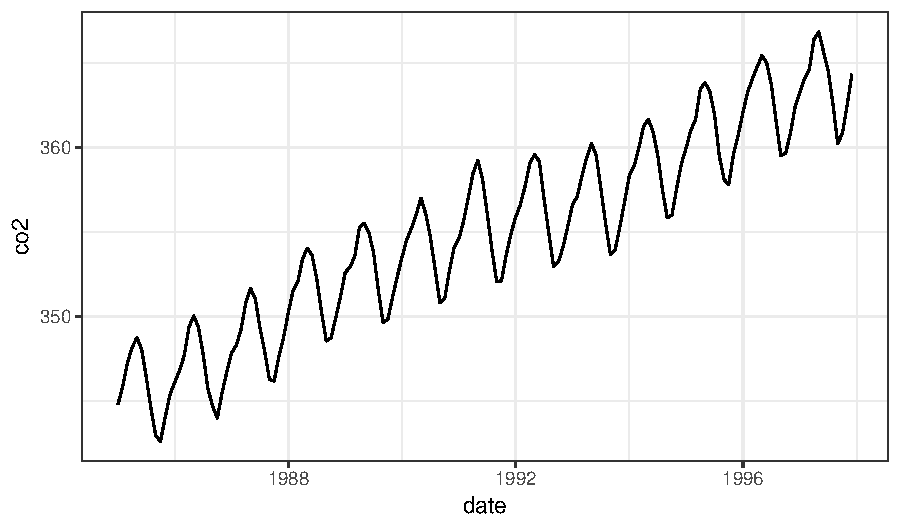
\includegraphics{Lec3_files/figure-beamer/unnamed-chunk-1-1.pdf}

\end{frame}

\begin{frame}{Where to start?}

Well, it looks like stuff is going up on average \ldots{}

\pause

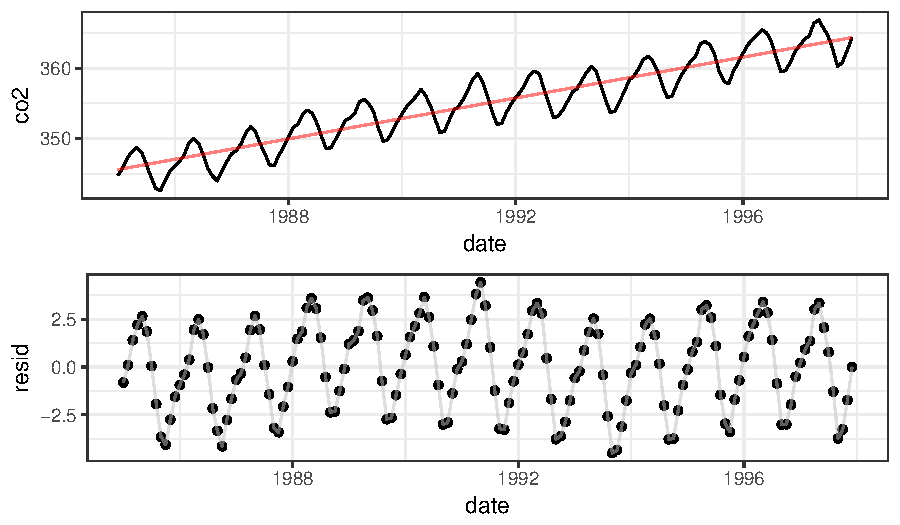
\includegraphics{Lec3_files/figure-beamer/unnamed-chunk-2-1.pdf}

\end{frame}

\begin{frame}{and then?}

Well there is some periodicity lets add the month \ldots{}

\pause

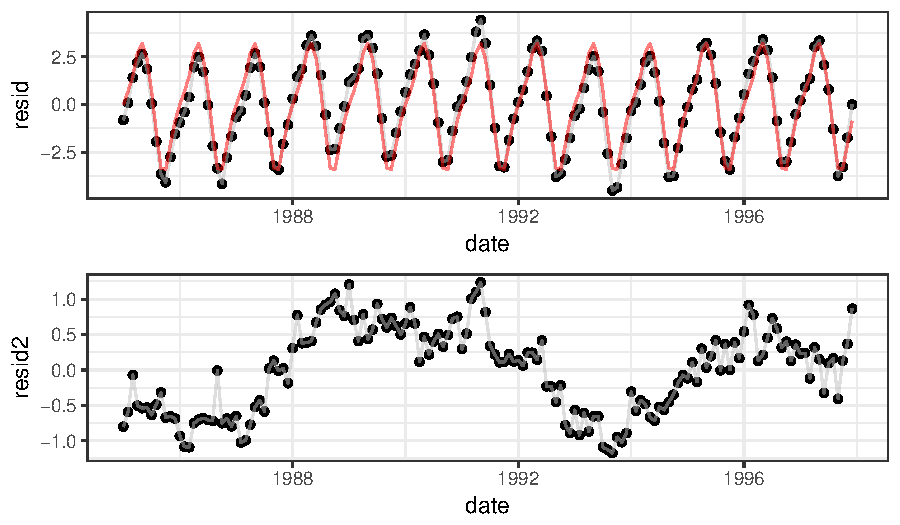
\includegraphics{Lec3_files/figure-beamer/unnamed-chunk-3-1.pdf}

\end{frame}

\begin{frame}{and then and then?}

Maybe there is some different effect by year \ldots{}

\pause

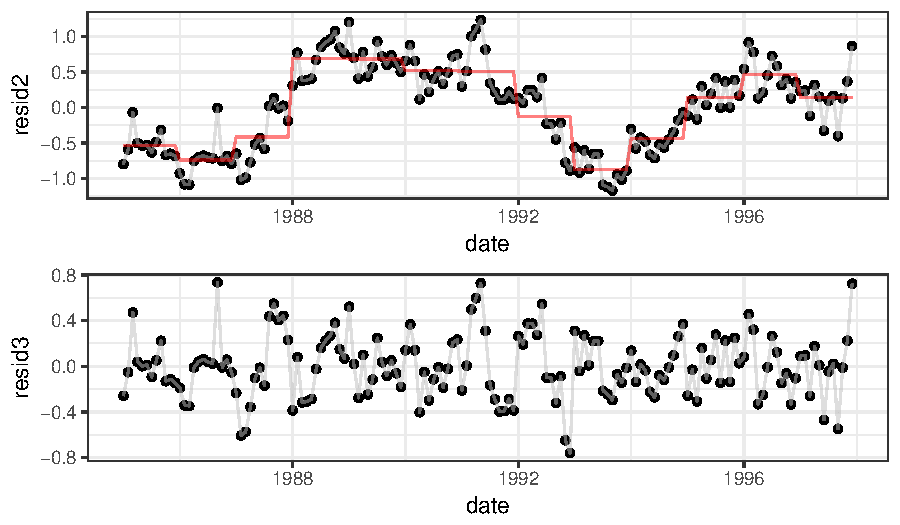
\includegraphics{Lec3_files/figure-beamer/unnamed-chunk-4-1.pdf}

\end{frame}

\begin{frame}[fragile]{Too much}

\begin{Shaded}
\begin{Highlighting}[]
\NormalTok{(}\DataTypeTok{lm =} \KeywordTok{lm}\NormalTok{(co2~date +}\StringTok{ }\NormalTok{month +}\StringTok{ }\KeywordTok{as.factor}\NormalTok{(year), }\DataTypeTok{data=}\NormalTok{co2_df))}
\NormalTok{## }
\NormalTok{## Call:}
\NormalTok{## lm(formula = co2 ~ date + month + as.factor(year), data = co2_df)}
\NormalTok{## }
\NormalTok{## Coefficients:}
\NormalTok{##         (Intercept)                 date             monthAug  }
\NormalTok{##          -2.645e+03            1.508e+00           -4.177e+00  }
\NormalTok{##            monthDec             monthFeb             monthJan  }
\NormalTok{##          -3.612e+00           -2.008e+00           -2.705e+00  }
\NormalTok{##            monthJul             monthJun             monthMar  }
\NormalTok{##          -2.035e+00           -3.251e-01           -1.227e+00  }
\NormalTok{##            monthMay             monthNov             monthOct  }
\NormalTok{##           4.821e-01           -4.838e+00           -6.135e+00  }
\NormalTok{##            monthSep  as.factor(year)1986  as.factor(year)1987  }
\NormalTok{##          -6.064e+00           -2.585e-01            9.722e-03  }
\NormalTok{## as.factor(year)1988  as.factor(year)1989  as.factor(year)1990  }
\NormalTok{##           1.065e+00            9.978e-01            7.726e-01  }
\NormalTok{## as.factor(year)1991  as.factor(year)1992  as.factor(year)1993  }
\NormalTok{##           7.067e-01            1.236e-02           -7.911e-01  }
\NormalTok{## as.factor(year)1994  as.factor(year)1995  as.factor(year)1996  }
\NormalTok{##          -4.146e-01            1.119e-01            3.768e-01  }
\NormalTok{## as.factor(year)1997  }
\NormalTok{##                  NA}
\end{Highlighting}
\end{Shaded}

\end{frame}

\begin{frame}{}

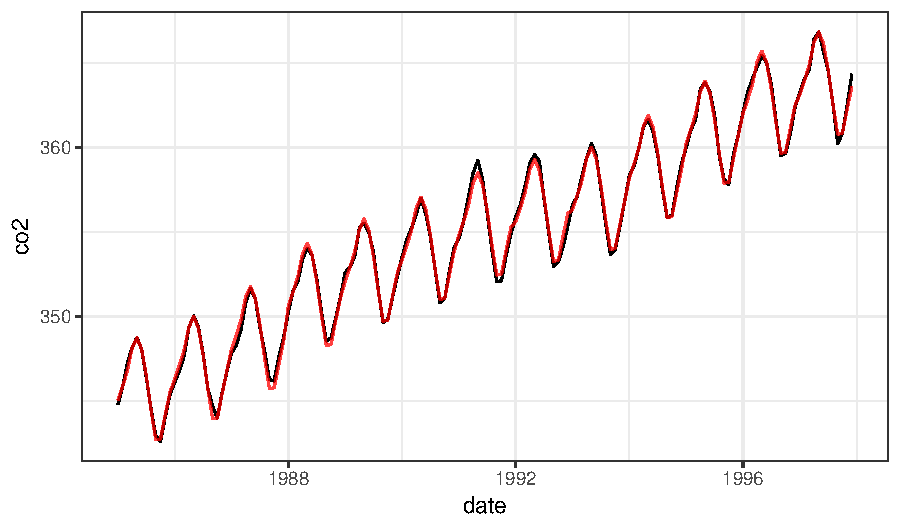
\includegraphics{Lec3_files/figure-beamer/unnamed-chunk-6-1.pdf}

\end{frame}

\section{Generalized Linear Models}\label{generalized-linear-models}

\begin{frame}{Background}

A generalized linear model has three key components:

\begin{enumerate}
\def\labelenumi{\arabic{enumi}.}
\item
  a probability distribution (from the exponential family) that
  describes your response variable
\item
  a linear predictor \(\bm{\eta} = \bm{X}\bm{\beta}\),
\item
  and a link function \(g\) such that
  \(g(E(\bm{Y}|\bm{X})) = \bm{\mu} = \bm{\eta}\).
\end{enumerate}

\end{frame}

\section{Poisson Regression}\label{poisson-regression}

\begin{frame}{Model Specification}

A generalized linear model for count data where we assume the outcome
variable follows a poisson distribution (mean = variance).

\[
\begin{aligned}
Y_i &\sim \text{Poisson}(\lambda_i)\\
 \log E(\bm{Y}|\bm{X}) &= \log{\bm{\lambda}} = \bm{X}\bm{\beta}
\end{aligned}
\]

\end{frame}

\begin{frame}{Example - AIDS in Belgium}

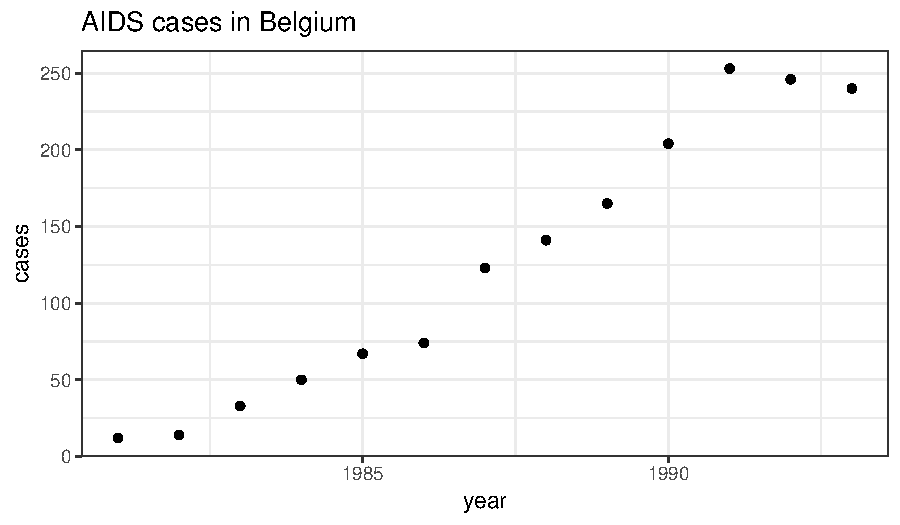
\includegraphics{Lec3_files/figure-beamer/unnamed-chunk-7-1.pdf}

\end{frame}

\begin{frame}[fragile]{Frequentist glm fit}

\begin{Shaded}
\begin{Highlighting}[]
\NormalTok{g =}\StringTok{ }\KeywordTok{glm}\NormalTok{(cases~year, }\DataTypeTok{data=}\NormalTok{aids, }\DataTypeTok{family=}\NormalTok{poisson)}
\NormalTok{pred =}\StringTok{ }\KeywordTok{data_frame}\NormalTok{(}\DataTypeTok{year=}\KeywordTok{seq}\NormalTok{(}\DecValTok{1981}\NormalTok{,}\DecValTok{1993}\NormalTok{,}\DataTypeTok{by=}\FloatTok{0.1}\NormalTok{))}
\NormalTok{pred$cases =}\StringTok{ }\KeywordTok{predict}\NormalTok{(g, }\DataTypeTok{newdata=}\NormalTok{pred, }\DataTypeTok{type =} \StringTok{"response"}\NormalTok{)}
\end{Highlighting}
\end{Shaded}

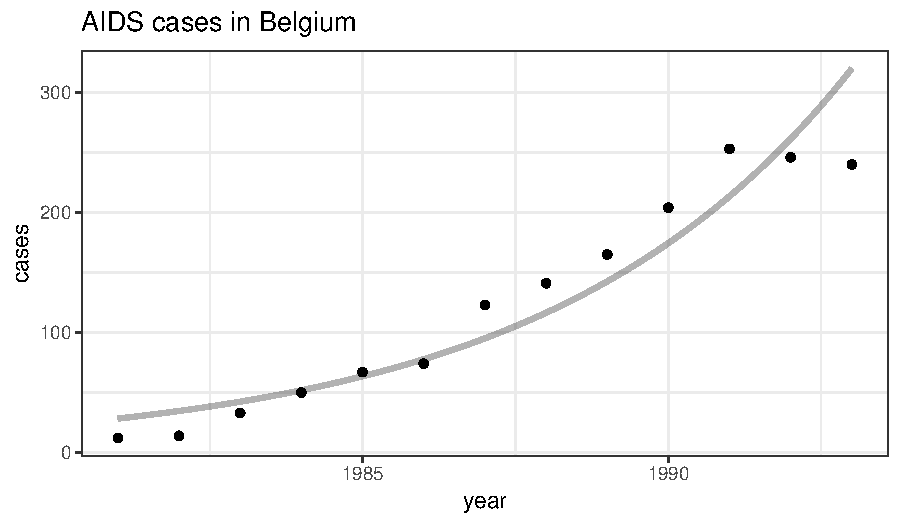
\includegraphics{Lec3_files/figure-beamer/unnamed-chunk-9-1.pdf}

\end{frame}

\begin{frame}{Residuals}

Standard residuals:

\[ r_i = Y_i - \hat{Y}_i = Y_i - \hat\lambda_i\] Pearson residuals:

\[ r_i = \frac{Y_i - E(Y_i|X)}{\sqrt{Var(Y_i|X)}} = \frac{Y_i - \hat\lambda_i}{\sqrt{\hat\lambda_i}}\]

Deviance residuals:

\[ d_i = \text{sign}(y_i - \lambda_i) \sqrt{2(y_i \log (y_i/\hat\lambda_i) - (y_i-\hat\lambda_i))}\]

\end{frame}

\begin{frame}{Deviance and deviance residuals}

Deviance can be interpreted as the difference between your model's fit
and the fit of an ideal model (where \(E(\hat{Y}_i) = Y_i\)).

\[ D = 2(\mathcal{L}(Y|\theta_{best}) - \mathcal{L}(Y|\hat\theta)) = \sum_{i=1}^n {d_i}^2 \]

Deviance is a measure of goodness of fit in a similar way to the
residual sum of squares (which is just the sum of squared standard
residuals).

\end{frame}

\begin{frame}{Deviance residuals derivation}

\end{frame}

\begin{frame}{Residual plots}

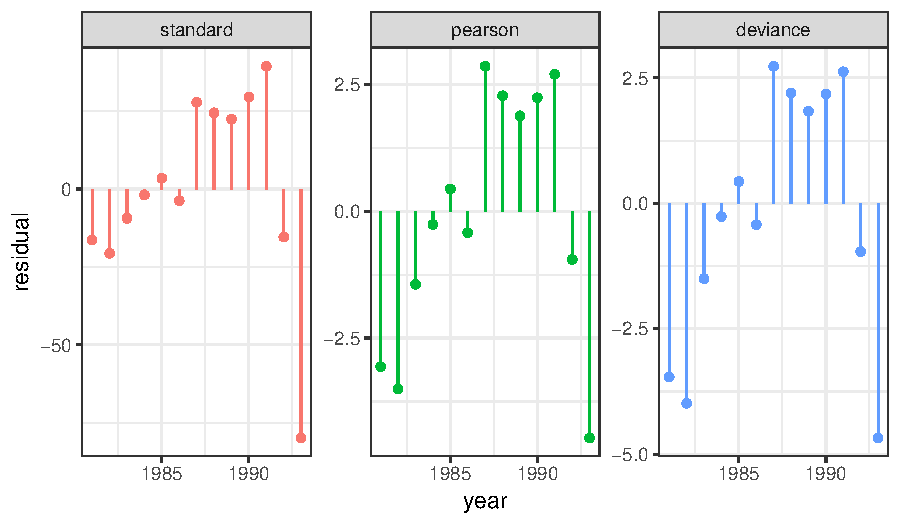
\includegraphics[width=\textwidth]{Lec3_files/figure-beamer/unnamed-chunk-11-1}

\end{frame}

\begin{frame}[fragile]{}

\begin{Shaded}
\begin{Highlighting}[]
\KeywordTok{print}\NormalTok{(aids_fit)}
\end{Highlighting}
\end{Shaded}

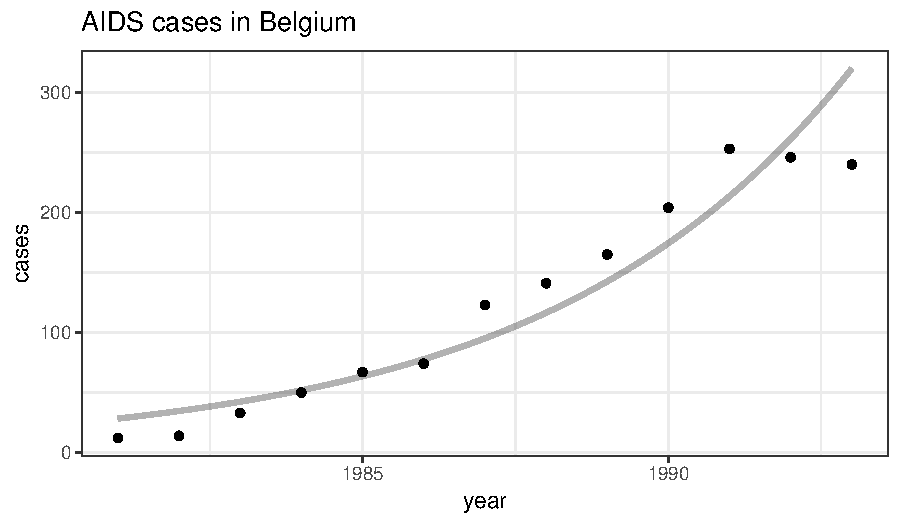
\includegraphics{Lec3_files/figure-beamer/unnamed-chunk-12-1.pdf}

\end{frame}

\begin{frame}[fragile]{Quadratic fit}

\begin{Shaded}
\begin{Highlighting}[]
\NormalTok{g2 =}\StringTok{ }\KeywordTok{glm}\NormalTok{(cases~year+}\KeywordTok{I}\NormalTok{(year^}\DecValTok{2}\NormalTok{), }\DataTypeTok{data=}\NormalTok{aids, }\DataTypeTok{family=}\NormalTok{poisson)}
\NormalTok{pred2 =}\StringTok{ }\KeywordTok{data_frame}\NormalTok{(}\DataTypeTok{year=}\KeywordTok{seq}\NormalTok{(}\DecValTok{1981}\NormalTok{,}\DecValTok{1993}\NormalTok{,}\DataTypeTok{by=}\FloatTok{0.1}\NormalTok{))}
\NormalTok{pred2$cases =}\StringTok{ }\KeywordTok{predict}\NormalTok{(g2, }\DataTypeTok{newdata=}\NormalTok{pred, }\DataTypeTok{type =} \StringTok{"response"}\NormalTok{)}
\end{Highlighting}
\end{Shaded}

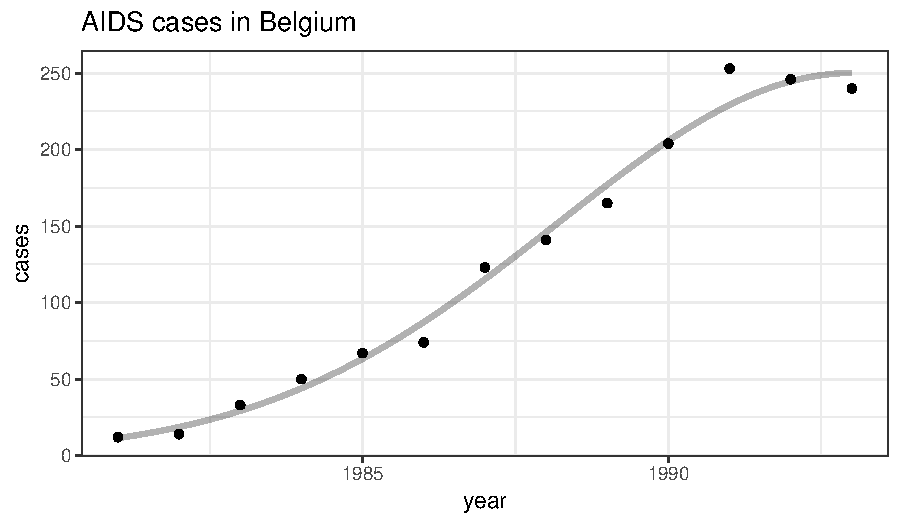
\includegraphics{Lec3_files/figure-beamer/unnamed-chunk-14-1.pdf}

\end{frame}

\begin{frame}{Quadratic fit - residuals}

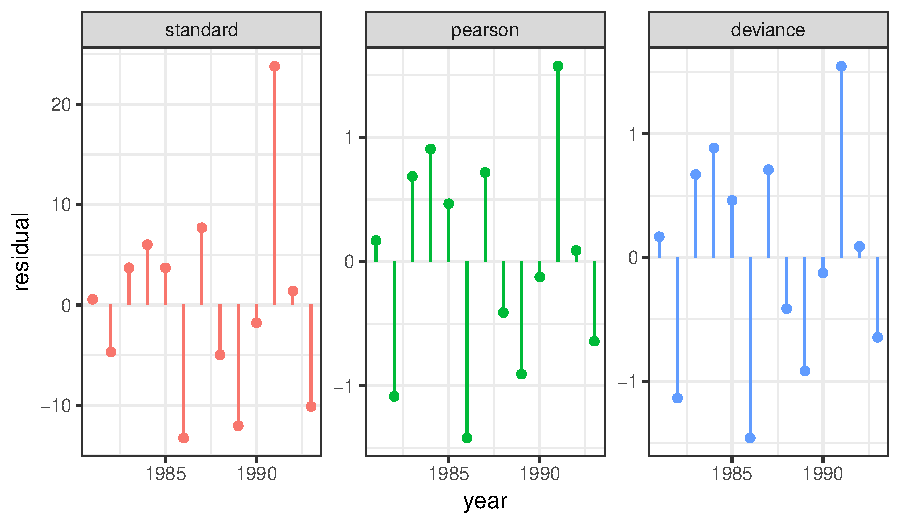
\includegraphics{Lec3_files/figure-beamer/unnamed-chunk-15-1.pdf}

\end{frame}

\begin{frame}[fragile]{Bayesian Poisson Regression Model}

\begin{verbatim}
## model{
##   # Likelihood
##   for(i in 1:length(Y)){
##     Y[i] ~ dpois(lambda[i])
##     log(lambda[i]) <- beta[1] + beta[2]*X[i]
##     
##     # In-sample prediction
##     Y_hat[i] ~ dpois(lambda[i])
##   }
## 
##   # Prior for beta
##   for(j in 1:2){
##     beta[j] ~ dnorm(0,1/100)
##   }
## }
\end{verbatim}

\end{frame}

\begin{frame}[fragile]{Bayesian Model fit}

\begin{Shaded}
\begin{Highlighting}[]
\NormalTok{m =}\StringTok{ }\KeywordTok{jags.model}\NormalTok{(}
  \KeywordTok{textConnection}\NormalTok{(poisson_model1), }\DataTypeTok{quiet =} \OtherTok{TRUE}\NormalTok{,}
  \DataTypeTok{data =} \KeywordTok{list}\NormalTok{(}\DataTypeTok{Y=}\NormalTok{aids$cases, }\DataTypeTok{X=}\NormalTok{aids$year)}
\NormalTok{) }
\KeywordTok{update}\NormalTok{(m, }\DataTypeTok{n.iter=}\DecValTok{1000}\NormalTok{, }\DataTypeTok{progress.bar=}\StringTok{"none"}\NormalTok{)}
\NormalTok{samp =}\StringTok{ }\KeywordTok{coda.samples}\NormalTok{(}
  \NormalTok{m, }\DataTypeTok{variable.names=}\KeywordTok{c}\NormalTok{(}\StringTok{"beta"}\NormalTok{,}\StringTok{"lambda"}\NormalTok{,}\StringTok{"Y_hat"}\NormalTok{), }
  \DataTypeTok{n.iter=}\DecValTok{5000}\NormalTok{, }\DataTypeTok{progress.bar=}\StringTok{"none"}
\NormalTok{)}
\end{Highlighting}
\end{Shaded}

\end{frame}

\begin{frame}{MCMC Diagnostics}

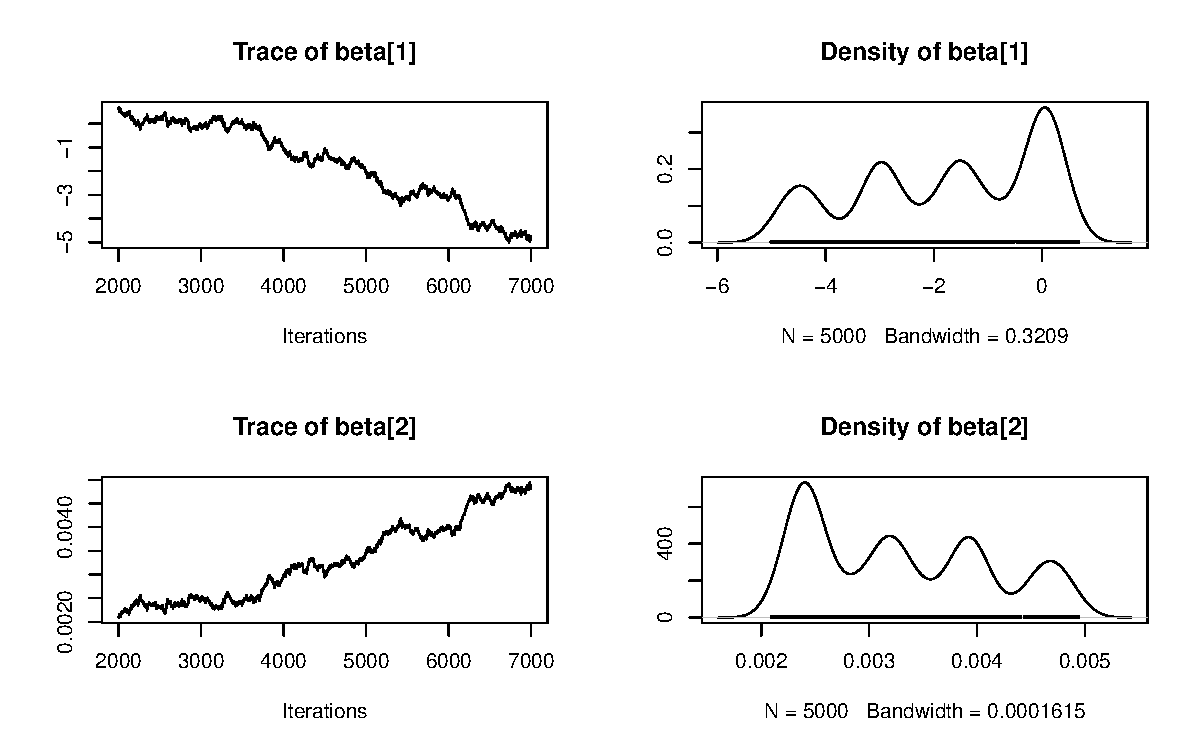
\includegraphics{Lec3_files/figure-beamer/unnamed-chunk-18-1.pdf}

\end{frame}

\begin{frame}{Model fit?}

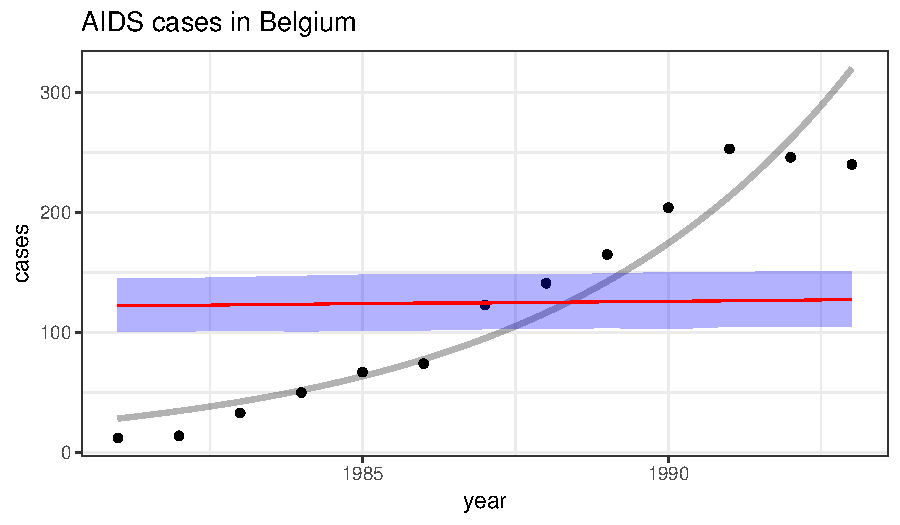
\includegraphics{Lec3_files/figure-beamer/unnamed-chunk-19-1.pdf}

\end{frame}

\begin{frame}[fragile]{What went wrong?}

\pause

\begin{Shaded}
\begin{Highlighting}[]
\KeywordTok{summary}\NormalTok{(g)}
\NormalTok{## }
\NormalTok{## Call:}
\NormalTok{## glm(formula = cases ~ year, family = poisson, data = aids)}
\NormalTok{## }
\NormalTok{## Deviance Residuals: }
\NormalTok{##     Min       1Q   Median       3Q      Max  }
\NormalTok{## -4.6784  -1.5013  -0.2636   2.1760   2.7306  }
\NormalTok{## }
\NormalTok{## Coefficients:}
\NormalTok{##               Estimate Std. Error z value Pr(>|z|)    }
\NormalTok{## (Intercept) -3.971e+02  1.546e+01  -25.68   <2e-16 ***}
\NormalTok{## year         2.021e-01  7.771e-03   26.01   <2e-16 ***}
\NormalTok{## ---}
\NormalTok{## Signif. codes:  0 '***' 0.001 '**' 0.01 '*' 0.05 '.' 0.1 ' ' 1}
\NormalTok{## }
\NormalTok{## (Dispersion parameter for poisson family taken to be 1)}
\NormalTok{## }
\NormalTok{##     Null deviance: 872.206  on 12  degrees of freedom}
\NormalTok{## Residual deviance:  80.686  on 11  degrees of freedom}
\NormalTok{## AIC: 166.37}
\NormalTok{## }
\NormalTok{## Number of Fisher Scoring iterations: 4}
\end{Highlighting}
\end{Shaded}

\end{frame}

\begin{frame}[fragile]{}

\begin{Shaded}
\begin{Highlighting}[]
\KeywordTok{summary}\NormalTok{(}\KeywordTok{glm}\NormalTok{(cases~}\KeywordTok{I}\NormalTok{(year}\DecValTok{-1981}\NormalTok{), }\DataTypeTok{data=}\NormalTok{aids, }\DataTypeTok{family=}\NormalTok{poisson))}
\NormalTok{## }
\NormalTok{## Call:}
\NormalTok{## glm(formula = cases ~ I(year - 1981), family = poisson, data = aids)}
\NormalTok{## }
\NormalTok{## Deviance Residuals: }
\NormalTok{##     Min       1Q   Median       3Q      Max  }
\NormalTok{## -4.6784  -1.5013  -0.2636   2.1760   2.7306  }
\NormalTok{## }
\NormalTok{## Coefficients:}
\NormalTok{##                Estimate Std. Error z value Pr(>|z|)    }
\NormalTok{## (Intercept)    3.342711   0.070920   47.13   <2e-16 ***}
\NormalTok{## I(year - 1981) 0.202121   0.007771   26.01   <2e-16 ***}
\NormalTok{## ---}
\NormalTok{## Signif. codes:  0 '***' 0.001 '**' 0.01 '*' 0.05 '.' 0.1 ' ' 1}
\NormalTok{## }
\NormalTok{## (Dispersion parameter for poisson family taken to be 1)}
\NormalTok{## }
\NormalTok{##     Null deviance: 872.206  on 12  degrees of freedom}
\NormalTok{## Residual deviance:  80.686  on 11  degrees of freedom}
\NormalTok{## AIC: 166.37}
\NormalTok{## }
\NormalTok{## Number of Fisher Scoring iterations: 4}
\end{Highlighting}
\end{Shaded}

\end{frame}

\begin{frame}[fragile]{Revising the model}

\begin{verbatim}
## model{
##   # Likelihood
##   for(i in 1:length(Y)){
##     Y[i] ~ dpois(lambda[i])
##     log(lambda[i]) <- beta[1] + beta[2]*(X[i] - 1981)
##     
##     # In-sample prediction
##     Y_hat[i] ~ dpois(lambda[i])
##   }
## 
##   # Prior for beta
##   for(j in 1:2){
##     beta[j] ~ dnorm(0,1/100)
##   }
## }
\end{verbatim}

\end{frame}

\begin{frame}{MCMC Diagnostics}

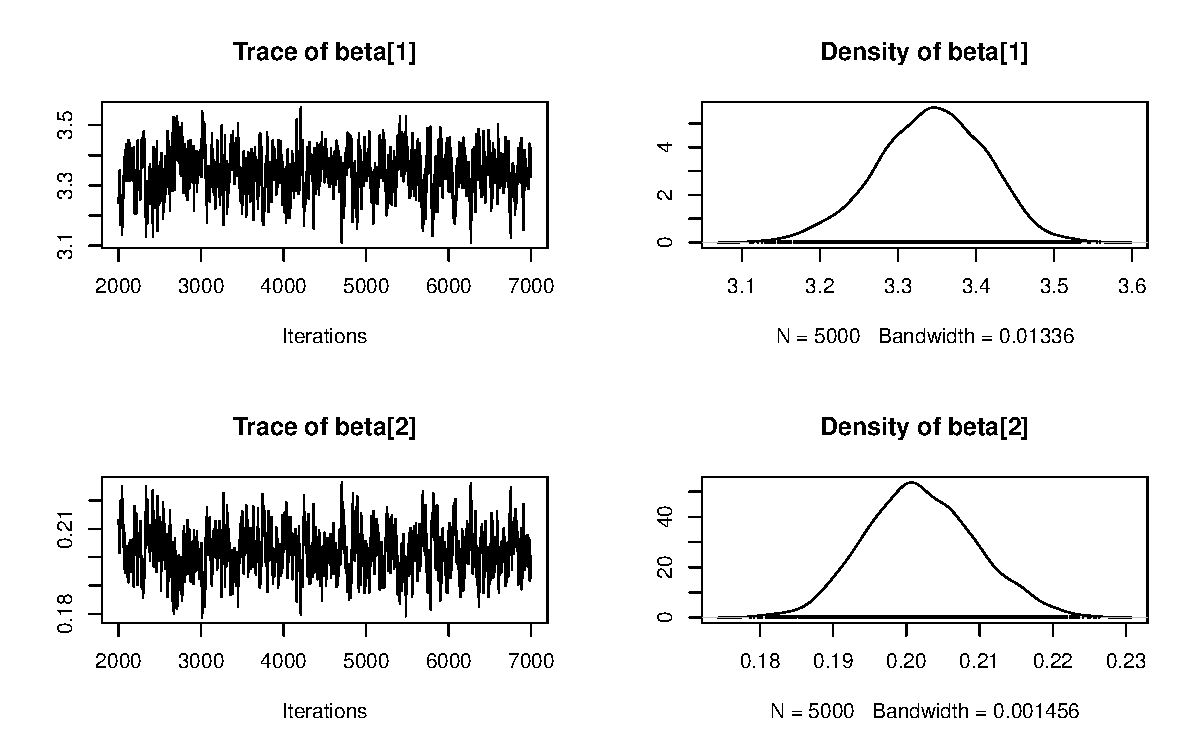
\includegraphics{Lec3_files/figure-beamer/unnamed-chunk-23-1.pdf}

\end{frame}

\begin{frame}{Model fit}

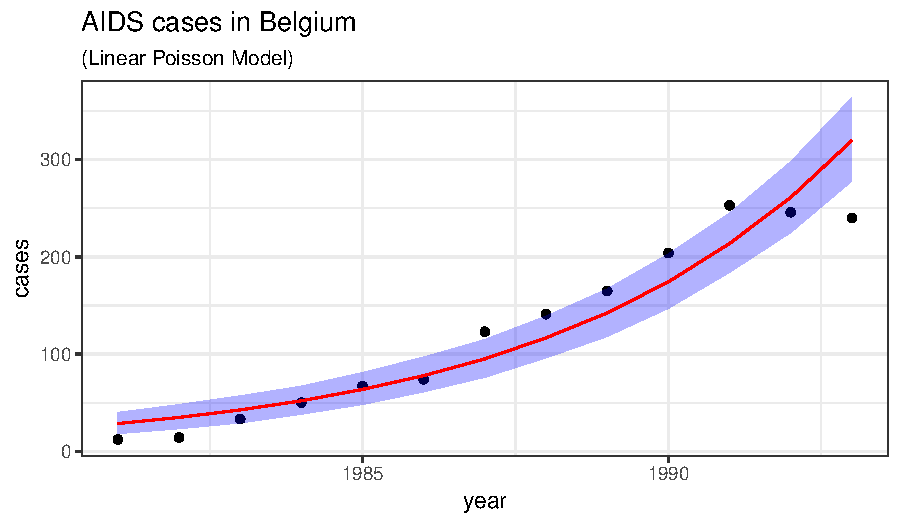
\includegraphics{Lec3_files/figure-beamer/unnamed-chunk-24-1.pdf}

\end{frame}

\begin{frame}{Bayesian Residual Plots}

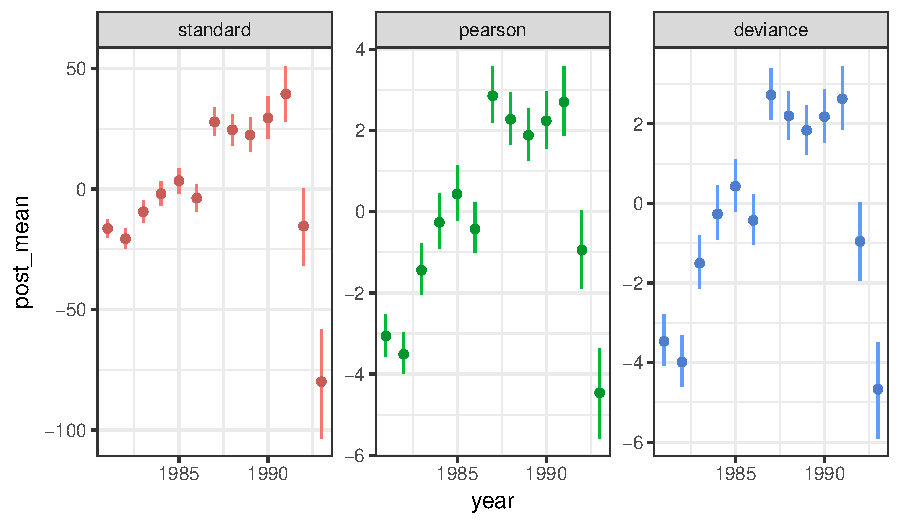
\includegraphics[width=\textwidth]{Lec3_files/figure-beamer/unnamed-chunk-25-1}

\end{frame}

\begin{frame}{Model fit}

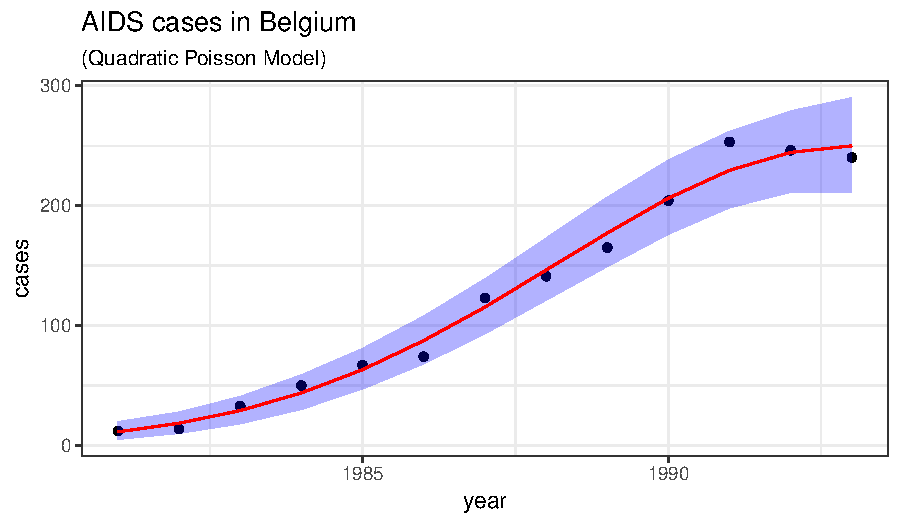
\includegraphics{Lec3_files/figure-beamer/unnamed-chunk-26-1.pdf}

\end{frame}

\begin{frame}{Bayesian Residual Plots}

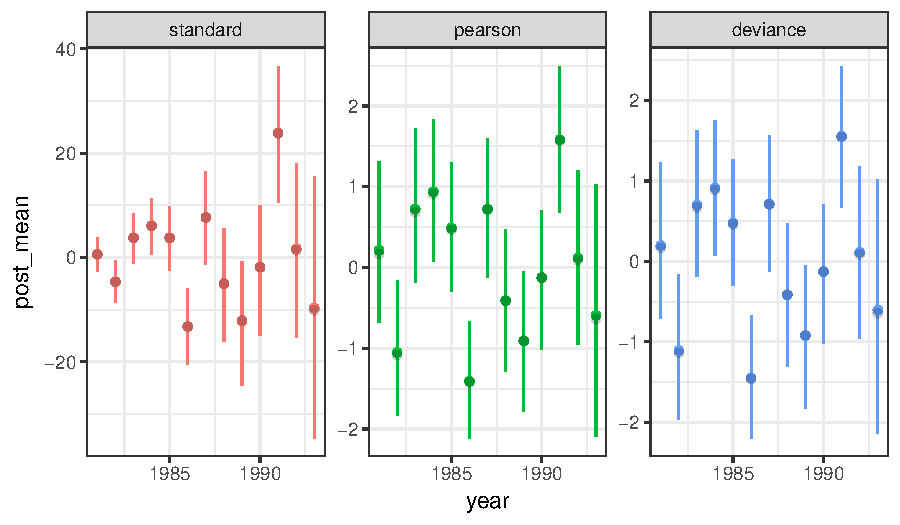
\includegraphics[width=\textwidth]{Lec3_files/figure-beamer/unnamed-chunk-27-1}

\end{frame}

\section{Negative Binomial
Regression}\label{negative-binomial-regression}

\begin{frame}[fragile]{Overdispersion}

One of the properties of the Poisson distribution is that if
\(X \sim \text{Pois}(\lambda)\) then \(E(X) = Var(X) = \lambda\).

If we are constructing a model where we claim that our response variable
\(Y\) follows a Poisson distribution then we are making a very strong
assumption which has implactions for both inference and prediction.

\pause

\begin{Shaded}
\begin{Highlighting}[]
\KeywordTok{mean}\NormalTok{(aids$cases)}
\NormalTok{## [1] 124.7692}
\KeywordTok{var}\NormalTok{(aids$cases)}
\NormalTok{## [1] 8124.526}
\end{Highlighting}
\end{Shaded}

\end{frame}

\begin{frame}{Negative binomial regession}

If we define

\[
\begin{aligned}
Y_i|Z_i &\sim \text{Pois}(\lambda_i \; Z_i) \\
Z_i &\sim \text{Gamma}(\theta_i, \, \theta_i)
\end{aligned}
\]

then the marginal distribution of \(Y_i\) will be negative binomial
with,

\[
\begin{aligned}
E(Y_i)   &= \lambda_i \\
Var(Y_i) &= \lambda_i + \lambda_i^2/\theta_i
\end{aligned}
\]

\end{frame}

\begin{frame}[fragile]{Model}

\begin{verbatim}
## model{
##   for(i in 1:length(Y))
##   {
##     Z[i] ~ dgamma(theta, theta)
##     log(lambda[i]) <- beta[1] + beta[2]*(X[i] - 1981) + beta[3]*(X[i] - 1981)^2
## 
##     lambda_Z[i] <- Z[i]*lambda[i]
## 
##     Y[i] ~ dpois(lambda_Z[i])
##     Y_hat[i] ~ dpois(lambda_Z[i])
##   }
## 
##   for(j in 1:3){
##     beta[j] ~ dnorm(0, 1/100)
##   }
## 
##   log_theta ~ dnorm(0, 1/100)
##   theta <- exp(log_theta)
## }
\end{verbatim}

\end{frame}

\begin{frame}{Negative Binomial Model fit}

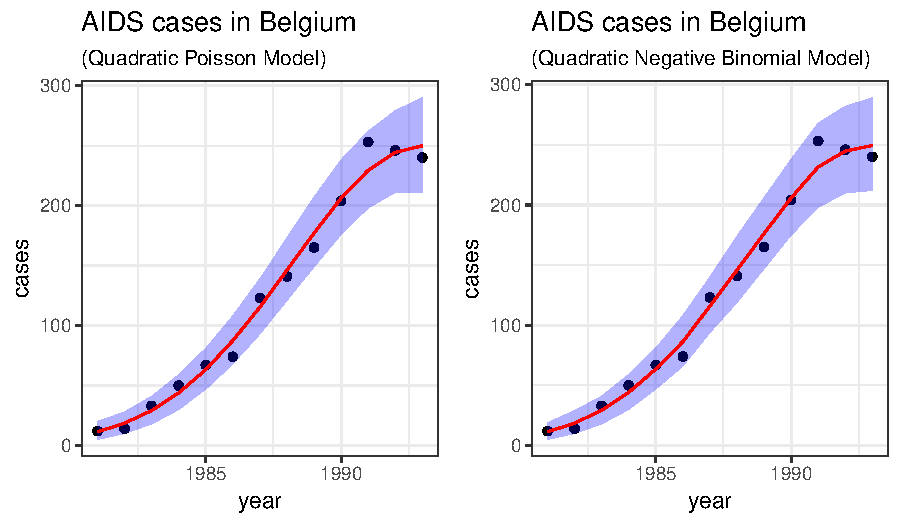
\includegraphics{Lec3_files/figure-beamer/unnamed-chunk-30-1.pdf}

\end{frame}

\begin{frame}{Bayesian Residual Plots}

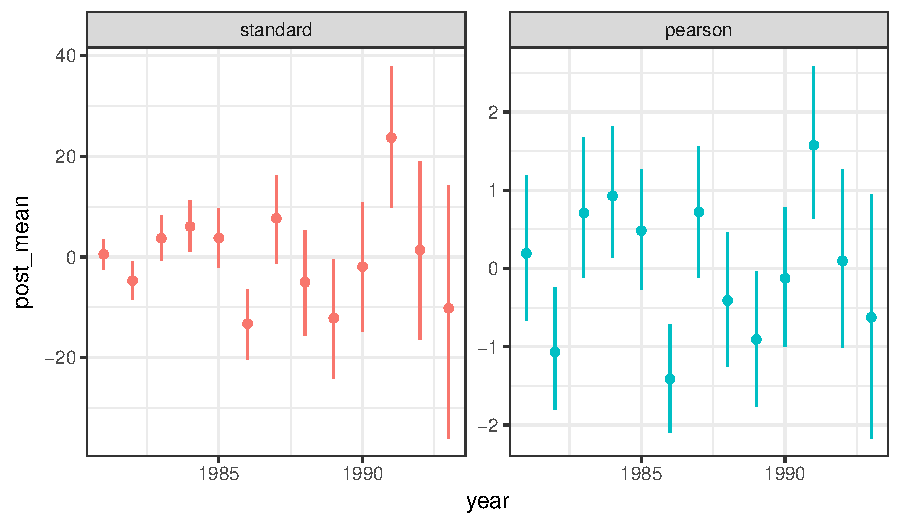
\includegraphics[width=\textwidth]{Lec3_files/figure-beamer/unnamed-chunk-31-1}

\end{frame}

\end{document}
